% Copyright 2004 by Till Tantau <tantau@users.sourceforge.net>.
%
% In principle, this file can be redistributed and/or modified under
% the terms of the GNU Public License, version 2.
%
% However, this file is supposed to be a template to be modified
% for your own needs. For this reason, if you use this file as a
% template and not specifically distribute it as part of a another
% package/program, I grant the extra permission to freely copy and
% modify this file as you see fit and even to delete this copyright
% notice. 

\documentclass{beamer}
% Replace the \documentclass declaration above
% with the following two lines to typeset your 
% lecture notes as a handout:
%\documentclass{article}
%\usepackage{beamerarticle}
\usepackage{graphicx}
\usepackage{natbib}
\usepackage{sansmathaccent}
\pdfmapfile{+sansmathaccent.map}
% There are many different themes available for Beamer. A comprehensive
% list with examples is given here:
% http://deic.uab.es/~iblanes/beamer_gallery/index_by_theme.html
% You can uncomment the themes below if you would like to use a different
% one:
%\usetheme{AnnArbor}
%\usetheme{Antibes}
%\usetheme{Bergen}
%\usetheme{Berkeley}
%\usetheme{Berlin}
\usetheme{Boadilla}
%\usetheme{boxes}
%\usetheme{CambridgeUS}
%\usetheme{Copenhagen}
%\usetheme{Darmstadt}
%\usetheme{default}
%\usetheme{Frankfurt}
%\usetheme{Goettingen}
%\usetheme{Hannover}
%\usetheme{Ilmenau}
%\usetheme{JuanLesPins}
%\usetheme{Luebeck}
%\usetheme{Madrid}
%\usetheme{Malmoe}
%\usetheme{Marburg}
%\usetheme{Montpellier}
%\usetheme{PaloAlto}
%\usetheme{Pittsburgh}
%\usetheme{Rochester}
%\usetheme{Singapore}
%\usetheme{Szeged}
%\usetheme{Warsaw}

\title{Macroprudential Policies and Capital Structure: \\Evidence from Multinationals}

% A subtitle is optional and this may be deleted
%\subtitle{Gauti B. Eggertsson and Paul Krugman}
\author{Lucas Avezum}

%\author{F.~Author\inst{1} \and S.~Another\inst{2}}
% - Give the names in the same order as the appear in the paper.
% - Use the \inst{?} command only if the authors have different
%   affiliation.

%\institute[Universities of Somewhere and Elsewhere] % (optional, but mostly needed)
%{
 % \inst{1}%
  %Department of Computer Science\\
  %University of Somewhere
  %\and
  %\inst{2}%
  %Department of Theoretical Philosophy\\
  %University of Elsewhere}
% - Use the \inst command only if there are several affiliations.
% - Keep it simple, no one is interested in your street address.

\date{09/10/2017}
% - Either use conference name or its abbreviation.
% - Not really informative to the audience, more for people (including
%   yourself) who are reading the slides online

%\subject{Theoretical Computer Science}
% This is only inserted into the PDF information catalog. Can be left
% out. 

% If you have a file called "university-logo-filename.xxx", where xxx
% is a graphic format that can be processed by latex or pdflatex,
% resp., then you can add a logo as follows:

% \pgfdeclareimage[height=0.5cm]{university-logo}{university-logo-filename}
% \logo{\pgfuseimage{university-logo}}

% Delete this, if you do not want the table of contents to pop up at
% the beginning of each subsection:
%\AtBeginSubsection[]
%{
%  \begin{frame}<beamer>{Outline}
%    \tableofcontents[currentsection,currentsubsection]
%  \end{frame}
%}

% Let's get started
\begin{document}
	\begin{frame}
	\titlepage
\end{frame}

\begin{frame}{Introduction}{Quantity and intensity of macroprudential policies}

\begin{figure} [h!]
	\centering

	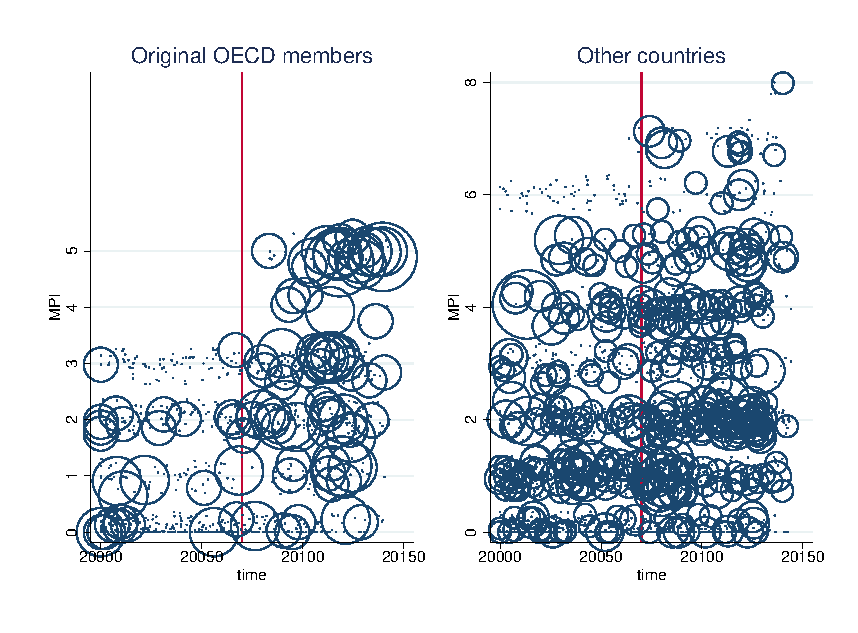
\includegraphics[scale=0.75]{C:/Users/u1273941/Research/Projects/macroprudential_capital_structure/analysis/output/graphs/intensity_graphs.eps}
	
\end{figure}

\end{frame}

\begin{frame}{Introduction}{Motivation}
\begin{itemize}
	\item Increasingly used by Central Banks  (\cite*{NBERw22735})
	\item Effectiveness and spillover still to be fully evaluated
\item	\cite*{jimenez2012macroprudential}, 
	\cite*{aiyar2014does}
	 \cite*{buch2017cross}
	\cite*{ayyagari2017credit},
	\item Our contribution: if and how macroprudential policies affect non-financial firms' capital structure
		
\end{itemize}
\end{frame}

\begin{frame}{Introduction}{Results}
\begin{itemize}
	\item Using a firm-level dataset of multinationals hosted in 37 countries we are able to identify domestic and international effects.
	\item Tighter capital requirements reduce firms' leverage while multinationals have an extra incentive to shift debt due to moves in reserve requirements. Moreover, the domestic effect is found to be stronger for riskier firms.
\end{itemize}
\end{frame}

\begin{frame}{Model}{Balance sheets and financial leverage}
Based on \cite*{huizinga2008capital}
\begin{itemize}
	\item  Balance sheet:
\end{itemize}
\begin{equation}
\begin{aligned}
A_i=I_i+L_i, \quad i=1,...,n-1.
\end{aligned}
\label{eq:sub balance sheet}
\end{equation}
\begin{equation}
\begin{aligned}
A_p+\sum_{i=1}^{n-1}I_i=E_p+L_p. 
\end{aligned}
\label{eq:parent balance sheet}
\end{equation}
\begin{itemize}
	\item  Financial leverage:
\end{itemize}
\begin{equation*}
\begin{aligned}
\lambda_i=L_i/A_i, \quad i=1,...,n-1.
\end{aligned}
\label{eq:sub leverage}
\end{equation*}
\begin{equation}
\begin{aligned}
\lambda_m=\frac{\sum_{i=1}^{n}L_i}{\sum_{i=1}^{n}A_i}=\sum_{i=1}^{n}\lambda_i\rho_i, 
\end{aligned}
\label{eq:total leverage}
\end{equation} 
\end{frame}

\begin{frame}{Model}{Costs associated with leverage}
\begin{itemize}
	\item  Expected cost of bankruptcy:
\end{itemize}
\begin{equation}
\begin{aligned}
C_m=\frac{\gamma}{2}\lambda_m^2\bigg(\sum_{i=1}^{n}A_i\bigg).
\end{aligned}
\label{eq:cost bankruptcy}
\end{equation}
\begin{itemize}
\item  Costs associated to incentives to local managers:
\end{itemize}
\begin{equation}
\begin{aligned}
C_i=\frac{\mu}{2}(\lambda_i-\lambda^*)^2A_i-\frac{\mu}{2}(\lambda^*)^2A_i, \quad i=1,...,n.
\end{aligned}
\label{eq:agency cost}
\end{equation}
\begin{itemize}
	\item  Cost of debt:
\end{itemize}
\begin{equation}
\begin{aligned}
r_i=\delta_i(1+\phi'\Pi_i)
\end{aligned}
\label{eq:cost of debt}
\end{equation}
\begin{equation}
\phi'\Pi=\begin{bmatrix}
\phi_{rr} &  \phi_{cb}
\end{bmatrix}
\begin{bmatrix}
\Pi_{rr} \\   
\Pi_{cr} 
\end{bmatrix}
\label{eq:phi vector}
\end{equation}
\end{frame}

\begin{frame}{Model}{Multinational's value}
\begin{itemize}
	\item  Unleveraged firm's value:
\end{itemize}
\begin{equation}
\begin{aligned}
V_i^U=\frac{R_i}{\delta_i}(1-\tau_{i}),  \quad i=1,...,n.
\end{aligned}
\label{eq:v_u}
\end{equation}
\begin{itemize}
	\item Leverage firm's value:
\end{itemize}
\begin{equation}
\begin{aligned}
V_i^L=L_i+\frac{(R_i-r_iL_i)}{\delta_i}(1-\tau_{i})-C_i,  \quad i=1,...,n.
\end{aligned}
\label{eq:v_l_1}
\end{equation}
\begin{equation}
\begin{aligned}
V_i^L=V_i^U+\tau_{i}L_i-\phi'\Pi_iL_i+\tau_{i}\phi'\Pi_iL_i-C_i,  \quad i=1,...,n.
\end{aligned}
\label{eq:v_l_2}
\end{equation}	
\begin{itemize}
	\item Multinational's value:
\end{itemize}
\begin{equation}
\begin{aligned}
V_m^L=V_m^U+\sum_{i=1}^{n}\tau_iL_i-\phi'\sum_{i=1}^{n}\Pi_iL_i+\phi'\sum_{i=1}^{n}\tau_i\Pi_i L_i-C_m-\sum_{i=1}^{n}C_i
\end{aligned}
\label{eq:v_l}
\end{equation}
\end{frame}

\begin{frame}{Model}{Optimal leverage}
\begin{itemize}
	\item  Multinational's problem:
\end{itemize}
	\begin{equation}
\begin{aligned}
\max_{L_i}V_m^L, \quad i=1,...,n.
\end{aligned}
\label{eq:problem}
\end{equation}
\begin{itemize}
	\item  First order conditions:
\end{itemize}
\begin{equation}
\begin{aligned}
\tau_i-\phi'\Pi_i+\phi'\Pi_i\tau_{i}-\gamma\lambda_m-\mu(\lambda_i-\lambda^*)=0, \quad i=1,...,n\\
\end{aligned}
\label{eq:FOC}
\end{equation}
\begin{equation}
\mu\lambda_i=\mu\lambda^*+\tau_{i}-\phi'\Pi_i+\phi'\Pi_i\tau_{i}-\gamma \sum_{j=1}^{n}\lambda_j\rho_j, \quad i=1,...,n
\label{eq:FOC2}
\end{equation}
\begin{itemize}
	\item Subtracting the first order condition for a subsidiary $j$ from the first order condition for a subsidiary $i$:
\end{itemize}
\begin{equation}
\begin{aligned}
\lambda_j=\lambda_i-\frac{1}{\mu}(\tau_i-\tau_j)+\frac{\phi'}{\mu}(\Pi_i-\Pi_j)-\frac{\phi'}{\mu}(\Pi_i\tau_i-\Pi_j\tau_j).
\end{aligned}
\label{eq:joint FOC}
\end{equation}
\end{frame}

\begin{frame}{Model}{Optimal leverage}
\begin{itemize}
	\item  Optimal leverage:
\end{itemize}
\begin{equation}
\begin{aligned}
\lambda_i = &\theta_0\lambda^*+\theta_1\tau_i-\theta_2\Pi_i+\theta_2\Pi_i\tau_{i}\\
&+\theta_3\sum_{j=1}^{n}(\tau_i-\tau_j)\rho_j-\theta_4\sum_{j=1}^{n}(\Pi_i-\Pi_j)\rho_j\\
&+\theta_4\sum_{j=1}^{n}(\Pi_i\tau_i-\Pi_j\tau_j)\rho_j, \quad i=1,...,n
\end{aligned}
\label{eq:optimal leverage in theory}
\end{equation}
\begin{equation*}
\begin{aligned}
&\theta_0=\frac{\mu}{(\mu+\gamma)}, \ \theta_1=\frac{1}{(\mu+\gamma)}, \
\theta_2=\frac{1}{(\mu+\gamma)}\phi', \\
&\theta_3=\frac{\gamma}{\mu(\mu+\gamma)}, \
\theta_4=\frac{\gamma}{\mu(\mu+\gamma)}\phi'.
\end{aligned}
\end{equation*}
\end{frame}

\begin{frame}{Data}
\begin{itemize}
	\item \cite{cerutti2017changes} for the measures of macroprudential policies 
	\item Orbis database compiled by Bureau Van Dijk for firm level data.
\end{itemize}
\begin{center}
		\begin{tiny}		\begin{table}[htbp]\centering
\begin{tabular}{l*{1}{cccccc}}
	\multicolumn{7}{c}{Summary statistics of leverage, macroprudential indexes and controls}\\
\hline\hline
                    &\multicolumn{6}{c}{}                                                         \\
                    &       Observation&        Mean&          SD&         Min&         Median&         Max\\
\hline
Financial leverage  &      443,941&        1.09&        1.07&        0.00&        0.98&       13.41\\
Reserve requirement &      443,941&       -0.43&        0.70&       -6.00&        0.00&        8.25\\
Capital requirement &      443,941&        0.54&        0.70&        0.00&        0.00&        2.00\\
Tax rate            &      443,930&        0.96&        0.08&        0.62&        0.99&        1.54\\
Reserve requirement spillover&      443,941&       -0.11&        0.51&       -7.88&        0.00&        8.89\\
Capital requirement spillover&      443,941&        0.01&        0.17&       -2.00&        0.00&        1.92\\
Tax rate spillover  &      443,941&       -0.01&        0.06&       -0.59&       0.00&        0.58\\
Tangibility         &      443,941&        1.48&        2.35&        0.00&        1.00&       19.06\\
Log of fixed assets &      443,941&        1.00&        0.08&        0.70&        1.00&        1.40\\
Profitability       &      443,941&        0.75&        3.91&      -22.24&        0.78&       23.32\\
Opportunity         &      443,941&       -0.02&        0.10&       -0.43&       -0.01&        0.34\\
Risk                &      443,941&        0.08&        0.13&        0.00&        0.05&        1.96\\
Inflation rate      &      443,906&        0.02&        0.02&       -0.01&        0.02&        0.22\\
GDP growth rate     &      443,941&        0.00&        0.03&       -0.15&        0.01&        0.10\\
Private credit to GDP&      443,927&        1.03&        0.12&        0.39&        1.04&        1.59\\
Policy rate         &      408,265&        0.43&        0.35&        0.00&        0.32&        3.48\\
Political Risk      &      443,941&        0.96&        0.05&        0.84&        0.97&        1.07\\
Exchange rate risk  &      443,941&        1.00&        0.13&        0.10&        1.00&       10.00\\
Law and order       &      443,941&        1.00&        0.01&        0.67&        1.00&        1.33\\
\hline\hline
\end{tabular}
\end{table}

	\end{tiny}
\end{center}
\end{frame}

\begin{frame}{Empirical Method}
Result lead to the following regression equation:
\begin{equation}
\begin{aligned}
\lambda_{imc(i),t}=&\alpha_0\tau_{c(i),t}+\beta_0\Pi_{c(i),t}+\beta_1\tau_{c(i),t}\Pi_{c(i),t}+\beta_3\sigma_{i}\Pi_{c(i),t}\\
&+\alpha_1\sum_{j=1}^{n}(\tau_{c(i),t}-\tau_{c(j),t})\rho_{j,t}+\beta_2\sum_{j=1}^{n}(\Pi_{c(i),t}-\Pi_{c(j),t})\rho_{j,t}\\
&+\Gamma_1 X_{i,t}+\Gamma_2 X_{c(i),t}+f_{...}+\varepsilon_{i,t},
\label{eq:optimal leverage empirically 1}
\end{aligned}
\end{equation}
Hypotheses:
\begin{itemize}
	\item H1: $\beta_0<0$ ($\beta_1>0$) 
	\item H2: $\beta_2<0$ and $\beta_3<0$
\end{itemize}
\end{frame}


\begin{frame}{Results}
\begin{center}
	\begin{tiny}		\begin{tabular}{lcccc}
\multicolumn{5}{c}{Effect of macroprudential policies on firm's financial leverage} \\ \hline
Model & (1) & (2) & (3) & (4) \\ \hline
 &  &  &  &  \\
Capital requirement & -0.103** & -0.088** &  &  \\
 & (0.041) & (0.041) &  &  \\
Reserve requirement & -0.056* & -0.043 &  &  \\
 & (0.029) & (0.029) &  &  \\
Capital requirement*tax & 0.120*** & 0.119*** &  &  \\
 & (0.039) & (0.039) &  &  \\
Reserve requirement*tax & 0.067** & 0.068** &  &  \\
 & (0.028) & (0.028) &  &  \\
Capital requirement spillover & -0.025* & -0.024* & -0.008 &  \\
 & (0.013) & (0.013) & (0.012) &  \\
Reserve requirement spillover & -0.021*** & -0.020** & -0.016* &  \\
 & (0.008) & (0.008) & (0.008) &  \\
Capital requirement*risk &  & -0.155*** & -0.148*** & -0.205*** \\
 &  & (0.055) & (0.054) & (0.061) \\
Reserve requirement*risk &  & -0.127* & -0.121* & -0.129* \\
 &  & (0.071) & (0.070) & (0.075) \\
Tax rate & 0.037 & 0.037 &  &  \\
 & (0.044) & (0.044) &  &  \\
Tax rate spillover & 0.174*** & 0.173*** & -0.023 &  \\
 & (0.047) & (0.047) & (0.041) &  \\
Risk & 0.073** & 0.085** & 0.092** & 0.112*** \\
 & (0.036) & (0.036) & (0.036) & (0.037) \\
  &  &  &  &  \\
Observations & 443,881 & 443,881 & 443,892 & 443,892 \\
Number of multinationals & 31,518 & 31,518 & 31,518 & 31,518 \\
Year fixed effects & Yes & Yes & No & No \\
Multinational fixed effects & Yes & Yes & Yes & No \\
Country*year fixed effects & No & No & Yes & Yes \\
 Multinational*year fixed effects & No & No & No & Yes \\ \hline

\end{tabular}

	\end{tiny}
\end{center}

\end{frame}

\begin{frame}{Results}
\begin{center}
	\begin{tiny}		\begin{tabular}{lcccc}
\multicolumn{5}{c}{Effect of macroprudential policies on firm's financial leverage} \\ \hline
Model  & (1) & (2) & (3) & (4) \\ \hline
 &  &  &  &  \\
Tangibility & -0.010** & -0.010** & -0.009** & -0.010** \\
 & (0.004) & (0.004) & (0.004) & (0.004) \\
Log of fixed assets & 1.074*** & 1.070*** & 1.066*** & 1.126*** \\
 & (0.100) & (0.101) & (0.101) & (0.110) \\
Profitability & -0.005*** & -0.005*** & -0.005*** & -0.006*** \\
 & (0.002) & (0.002) & (0.002) & (0.002) \\
Opportunity & 0.090*** & 0.091*** & 0.104*** & 0.139*** \\
 & (0.018) & (0.018) & (0.019) & (0.027) \\
Inflation rate & 0.429** & 0.407* &  &  \\
 & (0.217) & (0.216) &  &  \\
GDP growth rate & 0.365*** & 0.369*** &  &  \\
 & (0.108) & (0.108) &  &  \\
Private credit to GDP & 0.050 & 0.049 &  &  \\
 & (0.033) & (0.033) &  &  \\
Political Risk & -0.296*** & -0.292*** &  &  \\
 & (0.085) & (0.085) &  &  \\
Exchange rate risk & -0.040** & -0.041** &  &  \\
 & (0.017) & (0.017) &  &  \\
Law and order & 0.143 & 0.128 &  &  \\
 & (0.207) & (0.207) &  &  \\
 &  &  &  &  \\
Observations & 443,881 & 443,881 & 443,892 & 443,892 \\
Number of multinationals & 31,518 & 31,518 & 31,518 & 31,518 \\
Year fixed effects & Yes & Yes & No & No \\
Multinational fixed effects & Yes & Yes & Yes & No \\
Country*year fixed effects & No & No & Yes & Yes \\
 Multinational*year fixed effects & No & No & No & Yes \\ \hline
\end{tabular}

	\end{tiny}
\end{center}

\end{frame}

\begin{frame}{Results}
\begin{center}
	\begin{tiny}		\begin{tabular}{lcccc}
\multicolumn{5}{c}{Effect of macroprudential policies on firm's financial leverage: industry considerations} \\ \hline
Model & (1) & (2) & (3) & (4) \\ \hline
 &  &  &  &  \\
Capital requirement & -0.104** & -0.091** &  &  \\
 & (0.044) & (0.043) &  &  \\
Reserve requirement & -0.046 & -0.035 &  &  \\
 & (0.029) & (0.031) &  &  \\
Capital requirement*tax & 0.120*** & 0.119*** &  &  \\
 & (0.044) & (0.043) &  &  \\
Reserve requirement*tax & 0.056** & 0.056** &  &  \\
 & (0.027) & (0.027) &  &  \\
Capital requirement spillover & -0.025** & -0.024* & -0.009 &  \\
 & (0.013) & (0.013) & (0.013) &  \\
Reserve requirement spillover & -0.020*** & -0.019*** & -0.017** &  \\
 & (0.007) & (0.007) & (0.007) &  \\
Capital requirement*risk &  & -0.134* & -0.127* & -0.178** \\
 &  & (0.073) & (0.071) & (0.087) \\
Reserve requirement*risk &  & -0.117 & -0.110 & -0.116 \\
 &  & (0.084) & (0.082) & (0.095) \\
Risk & 0.149*** & 0.158*** & 0.160*** & 0.181*** \\
 & (0.038) & (0.039) & (0.039) & (0.044) \\
Tangibility & -0.008* & -0.008* & -0.008* & -0.008 \\
 & (0.004) & (0.004) & (0.004) & (0.005) \\

 &  &  &  &  \\
Observations & 440,568 & 440,568 & 440,573 & 440,573 \\
Industry*country clusters & 1,593 & 1,593 & 1,596 & 1,596 \\
Year fixed effects & Yes & Yes & No & No \\
Multinational fixed effects & Yes & Yes & Yes & No \\
Industry fixed effects & Yes & Yes & Yes & Yes \\
Country*year fixed effects & No & No & Yes & Yes \\
 Multinational*year fixed effects & No & No & No & Yes \\ \hline
\end{tabular}

	\end{tiny}
\end{center}
\end{frame}

\begin{frame}{Results}
\begin{center}
	\begin{tiny}		\begin{tabular}{lcc}
\multicolumn{3}{c}{Effect of macroprudential policies on firm's financial leverage: profitability considerations} \\ \hline
Model & No negative profitability & Only negative profitability \\ \hline
 &  &  \\
Capital requirement & -0.112*** & 0.049 \\
 & (0.037) & (0.153) \\
Reserve requirement & -0.036 & -0.014 \\
 & (0.027) & (0.112) \\
Capital requirement*tax & 0.109*** & 0.039 \\
 & (0.036) & (0.146) \\
Reserve requirement*tax & 0.049* & 0.044 \\
 & (0.027) & (0.102) \\
Capital requirement spillover & -0.007 & -0.106** \\
 & (0.012) & (0.052) \\
Reserve requirement spillover & -0.022*** & -0.024 \\
 & (0.007) & (0.036) \\
Capital requirement*risk & 0.055 & -0.490*** \\
 & (0.053) & (0.107) \\
Reserve requirement*risk & -0.028 & -0.213* \\
 & (0.061) & (0.125) \\
Tax rate & -0.022 & 0.278 \\
 & (0.047) & (0.174) \\
Tax rate spillover & 0.102** & 0.233 \\
 & (0.048) & (0.171) \\
Risk & 0.055* & 0.024 \\
 & (0.033) & (0.074) \\

 &  &  \\
Observations & 357,479 & 86,338 \\
Number of multinationals & 29,667 & 16,646 \\
Year fixed effects & Yes & Yes \\
Multinational fixed effects & Yes & Yes \\
 \hline
\end{tabular}

	\end{tiny}
\end{center}
\end{frame}

\begin{frame}{ Next Steps}
Theory on risk term:
\begin{itemize}
\item change equation \ref{eq:cost of debt} to $r_i=\delta_i(1+\phi'\sigma_{i}\Pi_i)$;
\item or build a second theory relating cost of debt and firms' riskiness   
\end{itemize}
Data issues:
\begin{itemize}
	\item Merge IBRN (\cite{cerutti2017changes}) to World Bank Regulation
	and Supervision Survey (\cite{barth2013bank})
\end{itemize}
Other spillover measures

\end{frame}

\begin{frame}{Conclusion}
\begin{itemize}
	\item Tighter capital requirements reduce firms' leverage while multinationals have an extra (weak) incentive to shift debt due to moves in reserve requirements. 
	\item The domestic effect is found to be stronger for riskier firms.

	
\end{itemize}
\end{frame}


\section{Bibliography}
\begin{frame}{Bibliography}{}
\begin{tiny}
\bibliography{C:/Users/u1273941/Research/Projects/macroprudential_capital_structure/analysis/code/text/bibliography/references}
\bibliographystyle{C:/Users/u1273941/Research/Projects/macroprudential_capital_structure/analysis/code/text/bibliography/te}
\end{tiny}
\end{frame}
\end{document}


